\documentclass[a4paper]{article}
\usepackage[utf8]{inputenc}
\usepackage[russian,english]{babel}
\usepackage[T2A]{fontenc}
\usepackage[left=10mm, top=20mm, right=18mm, bottom=15mm, footskip=10mm]{geometry}
\usepackage{indentfirst}
\usepackage{amsmath,amssymb}
\usepackage{mathastext} 

\usepackage[italicdiff]{physics}
\usepackage{graphicx}
\usepackage{caption}
\usepackage{float}
\usepackage{caption}
\renewcommand{\thefootnote}{\fnsymbol{footnote}}
\usepackage{tablefootnote}
\usepackage{footmisc}
\usepackage{textcomp}
\usepackage{multicol}
\usepackage[parfill]{parskip}
\usepackage{makecell}
\usepackage{array}  
\renewcommand\cellalign{cc} 
\renewcommand\cellgape{\Gape[2pt]} 
\usepackage[utf8]{inputenc}\newcommand{\approxtext}[1]{\ensuremath{\stackrel{\text{#1}}{\approx}}}
\usepackage[colorlinks=true, urlcolor=blue, linkcolor=blue, citecolor=blue]{hyperref}
\graphicspath{{images/}}
\DeclareGraphicsExtensions{.pdf,.png,.jpg}
\usepackage{wrapfig}
\captionsetup{labelformat=empty}
\usepackage{caption}
\captionsetup[figure]{name=Рисунок}
\captionsetup[table]{name=Таблица}
%\usepackage{newtxtext,newtxmath} 
\title{\textbf{Отчет о выполнении лабораторной работы 3.2.4-3.2.5}}
\date{}
\author{Котляров Михаил, Б01-402}

\begin{document}

\maketitle
	
	\section{Введение}
	
	\textbf{Цель работы:} Исследование свободных и вынужденных колебаний в колебательном контуре. В ходе работы необходимо:\\
\begin{itemize}
\item Изучить свободные колебания в электрическом контуре:
        \item Определить зависимость периода свободных колебаний контура от емкости.
        \item Определить зависимость логарифмического декремента затухания от сопротивления.
        \item Определить критическое сопротивление контура.
    \item Изучить вынужденные колебания в электрическом контуре:
    \item Построить резонансные кривые (АЧХ и ФЧХ) колебательного контура.
        \item Изучить процесс установления и затухания колебаний.
    \item Определить добротность контура различными способами.
\end{itemize}

	\textbf{Оборудование:} \begin{itemize}
\item Осциллограф АКТАКОМ ADS-6142H.
    \item Генератор сигналов специальной формы АКИП-3409/4.
    \item Магазин сопротивления МСР-60.
    \item Магазин емкости Р5025.
    \item Магазин индуктивности Р567 типа МИСП.
    \item Соединительная коробка с шунтирующей емкостью.
    \item Соединительные провода.
\end{itemize}
	\section{Теоретические сведения}

\subsection{Свободные колебания в RLC-контуре}
Рассмотрим последовательный RLC-контур, состоящий из резистора с сопротивлением $R$, катушки индуктивности $L$ и конденсатора с емкостью $C$. Для описания процессов в контуре применим второе правило Кирхгофа:

\begin{equation}
RI + U_C + L\frac{dI}{dt} = 0,
\label{eq:kirchhoff}
\end{equation}

где $I$ — ток в контуре, $U_C$ — напряжение на конденсаторе. Учитывая, что $I = C\frac{dU_C}{dt}$, подставим это выражение в уравнение (\ref{eq:kirchhoff}) и получим дифференциальное уравнение второго порядка для напряжения на конденсаторе:

\begin{equation}
\frac{d^2U_C}{dt^2} + \frac{R}{L}\frac{dU_C}{dt} + \frac{U_C}{LC} = 0.
\label{eq:diff_eq}
\end{equation}

Введем обозначения:
\begin{itemize}
\item $\gamma = \frac{R}{2L}$ — коэффициент затухания.
    \item $\omega_0^2 = \frac{1}{LC}$ — квадрат собственной (резонансной) частоты контура.
    \item $T_0 = \frac{2\pi}{\omega_0} = 2\pi\sqrt{LC}$ — период собственных незатухающих колебаний.
\end{itemize}

Тогда уравнение (\ref{eq:diff_eq}) можно записать в виде:

\begin{equation}
\ddot{U_C} + 2\gamma\dot{U_C} + \omega_0^2 U_C = 0.
\label{eq:diff_eq_simple}
\end{equation}

В зависимости от соотношения между $\gamma$ и $\omega_0$ возможны три режима колебаний:

\begin{enumerate}
    \item \textbf{Затухающие колебания ($\gamma < \omega_0$)}: Решение уравнения имеет вид:
    \begin{equation}
    U_C(t) = U_0 e^{-\gamma t} \cos(\omega_1 t + \varphi_0),
    \label{eq:free_oscillations}
    \end{equation}
    где $\omega_1 = \sqrt{\omega_0^2 - \gamma^2}$ — частота затухающих колебаний. Амплитуда колебаний убывает по экспоненциальному закону.

    \item \textbf{Критический режим ($\gamma = \omega_0$)}: Переходный режим, при котором система возвращается в состояние равновесия без колебаний за минимальное время. Решение имеет вид:
    \begin{equation}
    U_C(t) = (A + Bt)e^{-\gamma t}.
    \end{equation}

    \item \textbf{Апериодический режим ($\gamma > \omega_0$)}: Система возвращается в состояние равновесия без колебаний. Решение имеет вид суммы двух экспонент с разными постоянными времени.
\end{enumerate}

\subsection{Характеристики затухающих колебаний}
\begin{itemize}
\item \textbf{Логарифмический декремент затухания ($\Theta$)} определяется как натуральный логарифм отношения амплитуд двух соседних колебаний:
    \begin{equation}
    \Theta = \ln\left(\frac{U_k}{U_{k+1}}\right) = \gamma T_1,
    \end{equation}
    где $T_1 = \frac{2\pi}{\omega_1}$ — период затухающих колебаний. Также можно использовать формулу для амплитуд, разделенных $n$ периодами:
    \begin{equation}
    \Theta = \frac{1}{n} \ln\left(\frac{U_k}{U_{k+n}}\right).
    \end{equation}

    \item \textbf{Добротность контура ($Q$)} — важная характеристика, показывающая, насколько «острый» резонанс. Она связана с логарифмическим декрементом:
    \begin{equation}
    Q = \frac{\pi}{\Theta}.
    \end{equation}

    \item \textbf{Критическое сопротивление ($R_{cr}$)} — значение сопротивления, при котором происходит переход от колебательного режима к апериодическому. Оно рассчитывается по формуле:
    \begin{equation}
    R_{cr} = 2\sqrt{\frac{L}{C}}.
    \end{equation}
\end{itemize}
\subsection{Вынужденные колебания и резонанс}
При воздействии на контур внешней периодической ЭДС (например, синусоидальной) возникают вынужденные колебания. Уравнение движения в этом случае имеет вид:

\begin{equation}
\ddot{I} + 2\gamma\dot{I} + \omega_0^2 I = -\varepsilon_0 \frac{\Omega}{L} e^{i\Omega t},
\end{equation}

где $\varepsilon_0$ — амплитуда внешней ЭДС, $\Omega$ — частота вынуждающей силы. Решение этого уравнения представляет собой сумму затухающего переходного процесса и установившихся колебаний с частотой $\Omega$.
\begin{itemize}
\item \textbf{Резонанс} — явление резкого возрастания амплитуды вынужденных колебаний при приближении частоты вынуждающей силы к собственной частоте контура ($\Omega \approx \omega_0$).

    \item \textbf{Амплитудно-частотная характеристика (АЧХ)} — зависимость амплитуды напряжения на конденсаторе (или тока в контуре) от частоты вынуждающей силы. На резонансе амплитуда максимальна.

    \item \textbf{Фазово-частотная характеристика (ФЧХ)} — зависимость сдвига фаз между напряжением на конденсаторе и внешним напряжением от частоты. На резонансе сдвиг фаз равен $-\pi/2$.

    \item \textbf{Ширина резонансной кривой ($\Delta\Omega$)} — интервал частот, в пределах которого амплитуда колебаний не падает ниже $1/\sqrt{2}$ от максимального значения. Добротность контура можно определить по формуле:
    \begin{equation}
    Q = \frac{\omega_0}{\Delta\Omega}.
    \end{equation}
\end{itemize}
\subsection{Способы определения добротности}
В данной работе добротность контура определяется несколькими способами:

\begin{enumerate}
    \item По логарифмическому декременту затухания свободных колебаний: $Q = \pi / \Theta$.
    \item По ширине резонансной кривой (АЧХ): $Q = \omega_0 / \Delta\Omega$.
    \item По ФЧХ: Проводится горизонтальная линия на уровне $-\pi/2$, нижняя часть графика зеркально отражается относительно этой линии. Измеряется интервал частот $\Delta\omega$ на уровне $-\pi/4$. Тогда $Q = \omega_0 / \Delta\omega$.
\end{enumerate}

\section{Экспериментальная установка}

Экспериментальная установка предназначена для исследования свободных и вынужденных колебаний в параллельном колебательном контуре. Схема подключения приведена на рисунке~\ref{fig:scheme1}.

Колебательный контур состоит из:
\begin{enumerate}
\item постоянной индуктивности $L$ (магазин индуктивности Р567, $L = 100~\text{мГн}$), обладающей собственным активным сопротивлением $R_L$;
    \item переменной ёмкости $C$ (магазин ёмкости Р5025);
    \item регулируемого сопротивления $R$ (магазин сопротивления МСР-60).
\end{enumerate}

Возбуждение колебаний осуществляется с помощью генератора сигналов специальной формы АКИП-3409/4. Сигнал подаётся на вход контура через разделительный конденсатор $C_1$, который обеспечивает высокое выходное сопротивление генератора по постоянному току и исключает его влияние на параметры контура.

Напряжение с конденсатора $C$ подаётся на вход канала 1 (X) двухканального осциллографа АКТАКОМ ADS-6142H. Для наблюдения фазовой картины свободных колебаний на канал 2 (Y) подаётся напряжение с резистора $R$ (пунктирная линия на схеме), пропорциональное току в контуре: $U_R \propto I \propto dU_C/dt$.

При исследовании вынужденных колебаний генератор переключается в режим синусоидального сигнала, а его выход подаётся одновременно на колебательный контур и на канал 2 осциллографа (см. рисунок~\ref{fig:scheme2}), что позволяет измерять амплитудно-частотную (АЧХ) и фазово-частотную (ФЧХ) характеристики контура.

\begin{figure}[h]
    \centering
    % Здесь можно вставить изображение, если оно доступно:
    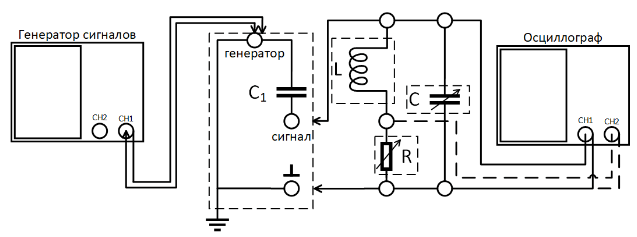
\includegraphics[width=0.8\textwidth]{Pictures/ustanovka1.png}
\caption{Рис. 1 Схема установки для исследования свободных и вынужденных колебаний}
\label{fig:scheme1}
\end{figure}

\begin{figure}[h]
    \centering
    
    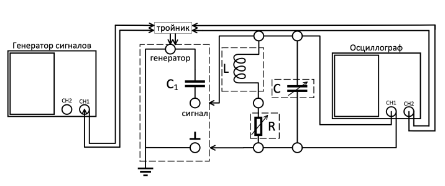
\includegraphics[width=0.8\textwidth]{Pictures/ustanovka2.png}
	\caption{Рис. 2 Схема подключения для снятия АЧХ и ФЧХ}
\label{fig:scheme2}
\end{figure}
\section{Выполнение}

\subsection{Подготовка приборов}
\begin{enumerate}
    \item Подключим генератор сигналов к входу канала 1 осциллографа.
    \item Установим на генераторе режим \texttt{Pulse} (импульсы):  
    длительность импульса — 10~мкс,  
    частота повторения — 100~Гц,  
    амплитуда — 20~В.  
    Включим выход генератора кнопкой \texttt{Output}.
    \item Настроим синхронизацию осциллографа по каналу 1 и получим устойчивое изображение импульсов (при необходимости воспользуемся кнопкой \texttt{Autoset}).
    \item Соберём схему согласно рисунку~\ref{fig:scheme1}: подключим колебательный контур к выходу генератора через разделительный конденсатор $C_1$, а напряжение с конденсатора $C$ — к каналу 1 осциллографа.
\end{enumerate}

\subsection{Измерение периода свободных колебаний}
\begin{enumerate}
    \item Установим на магазинах: $R = 0$, $L = 100~\text{мГн}$, $C = 0$ (минимальное 0,1 нФ).
    \item Наблюдая на экране осциллографа затухающие колебания, вызванные паразитной ёмкостью контура $C_0$, измерим период $T$ с помощью курсоров (расстояние между соседними максимумами). $T = 65$ мкс.
    \item По формуле $T = 2\pi\sqrt{L C_0}$ определим $C_0$. Получим $C_0 = 1,07$ нФ.
    \item Меняя ёмкость $C$ от 0 до 0.009~мкФ для 5–10 значений измерим соответствующие периоды $T$.

\begin{table}[h!]
    \centering
    \begin{tabular}{|c|c|c|}
        \hline
        $C,\ \text{нФ}$ & $T_{\text{эксп}},\ \text{мкс}$ & $T_{\text{теор}},\ \text{мкс}$ \\ \hline
        1 & $90{,}0 \pm 0{,}9$ & $90{,}40 \pm 0{,}14$ \\ \hline
        2 & $112{,}0 \pm 1{,}1$ & $110{,}09 \pm 0{,}17$ \\ \hline
        3 & $128{,}0 \pm 1{,}3$ & $126{,}76 \pm 0{,}19$ \\ \hline
        4 & $144{,}0 \pm 1{,}4$ & $141{,}48 \pm 0{,}21$ \\ \hline
        5 & $152{,}0 \pm 1{,}5$ & $154{,}80 \pm 0{,}23$ \\ \hline
        6 & $172{,}0 \pm 1{,}7$ & $167{,}07 \pm 0{,}25$ \\ \hline
        7 & $180{,}0 \pm 1{,}8$ & $178{,}49 \pm 0{,}27$ \\ \hline
        8 & $188{,}0 \pm 1{,}9$ & $189{,}23 \pm 0{,}28$ \\ \hline
    \end{tabular}
    \caption{Таблица 1. Сравнение экспериментальных и теоретических значений периода свободных колебаний.}
    \label{tab:periods_transposed}
\end{table}

Класс точности магазина емкостей равен 0,1, индуктивностей - 0,2. Поэтому погрешность теоретических периодов равна 0,15\%. Погрешность экспериментальных мы взяли за 1\%.
\item По МНК построим график $T_{\text{эксп}} = k  \cdot T_{\text{эксп}}$.
\clearpage
\begin{figure}[h]
        \center{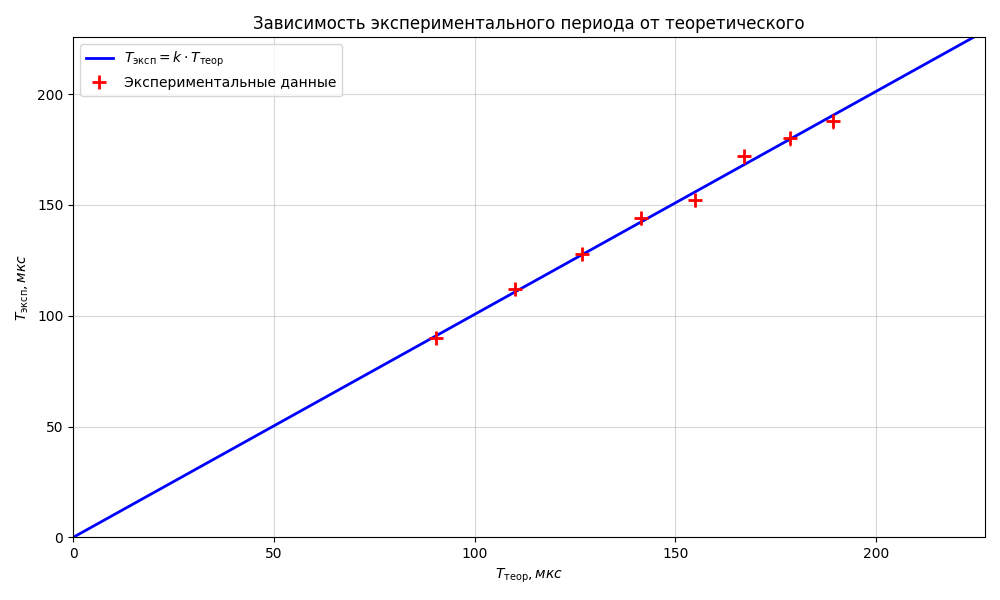
\includegraphics[width=1\textwidth]{Graphics/Texp_vs_Ttheor_plot.png}}
        \caption{График 1. Зависимость экспериментального периода от теоретического.}
\end{figure}

Коэффициент наклона $k = 1.006 \pm 0.006$ ($\varepsilon_k = 0,57 \%$). Как мы видим, в пределах погрешностей периоды совпадают.
\end{enumerate}

\subsection{Критическое сопротивление и логарифмический декремент}
\begin{enumerate}
    \item Рассчитаем требуемую ёмкость $C^*$ из условия $\nu_0 = 6.5~\text{кГц}$:  
    \[
        C^* = \frac{1}{(2\pi\nu_0)^2 L} = 5,995 \text{ нФ}.
    \]
    \item Вычислим теоретическое критическое сопротивление:  
    \[
        R_{\text{cr}} = 2\sqrt{\frac{L}{C^*}} = 8168 \text{ Ом}.
    \]
    \item Установим на магазине ёмкость, близкую к $C^*$, и, постепенно увеличивая $R$, определим экспериментальное значение $R_{\text{cr}}$ как границу перехода от колебательного режима к апериодическому. Получили, что $R_{\text{cr}} \approx 7 $ ÷ $ 8$ кОм.
    \item Установим $R \approx 0.05\,R_{\text{cr}}$, получим картину затухающих колебаний и измерим амплитуды $U_k$ и $U_{k+n}$, разделённые $n$ периодами.
    \item Рассчитаем логарифмический декремент по формуле:
    \[
        \Theta = \frac{1}{n} \ln\left(\frac{U_k}{U_{k+n}}\right).
    \]
    \item Повторим измерения для 6–8 значений $R$ в диапазоне $(0.05\text{–}0.25)R_{\text{cr}}$. Далее везде где будет использоваться сопротивление $R$, мы будем подразумевать $R_\Sigma = R + R_L$. Класс точности магазина сопротивлений 0,02. Омическое сопротивление магазина индуктивностей $R_L$ примем за 32 Ома, что соответствует верхнему порогу допустимого сопротивления между зажимами 1 и 2 согласно техническому описанию.

\begin{table}[h!]
    \centering
    \begin{tabular}{|c|c|c|c|c|c|c|}
        \hline
        $R_\Sigma,\ \Omega$ & $U_1,\ \text{В}$ & $U_{1+n},\ \text{В}$ & $n$ & $\Theta$ & $Q$ & $\varepsilon_Q,\ \%$ \\ \hline
        382 & $5{,}96 \pm 0{,}06$ & $1{,}60 \pm 0{,}02$ & 4 & $0{,}33 \pm 0{,}03$ & $9{,}56 \pm 0{,}94$ & 9{,}8 \\ \hline
        592 & $5{,}32 \pm 0{,}05$ & $0{,}76 \pm 0{,}01$ & 4 & $0{,}49 \pm 0{,}07$ & $6{,}46 \pm 0{,}88$ & 13{,}7 \\ \hline
        872 & $4{,}52 \pm 0{,}05$ & $0{,}44 \pm 0{,}00$ & 4 & $0{,}58 \pm 0{,}11$ & $5{,}39 \pm 1{,}06$ & 19{,}6 \\ \hline
        1232 & $3{,}68 \pm 0{,}04$ & $0{,}32 \pm 0{,}00$ & 3 & $0{,}81 \pm 0{,}21$ & $3{,}86 \pm 0{,}99$ & 25{,}7 \\ \hline
        1632 & $2{,}96 \pm 0{,}03$ & $0{,}40 \pm 0{,}00$ & 2 & $1{,}00 \pm 0{,}25$ & $3{,}14 \pm 0{,}79$ & 25{,}2 \\ \hline
        1782 & $2{,}72 \pm 0{,}03$ & $0{,}64 \pm 0{,}01$ & 1 & $1{,}45 \pm 0{,}32$ & $2{,}17 \pm 0{,}48$ & 22{,}2 \\ \hline
    \end{tabular}
    \caption{Таблица 2. Зависимость логарифмического декремента затухания и добротности от суммарного сопротивления контура.}
    \label{tab:theta_q_with_rel_error}
\end{table}

По этим данным по МНК построим график зависимости $\frac{1}{\Theta^2}(\frac{1}{R_\Sigma^2})$.

\begin{figure}[h]
        \center{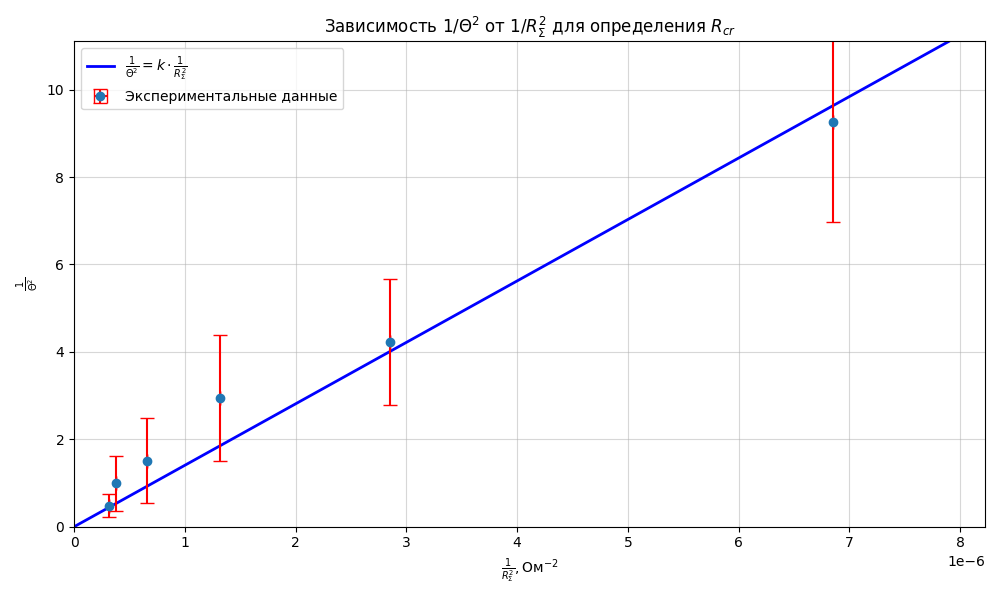
\includegraphics[width=1\textwidth]{Graphics/Decr_vs_RSigma_plot_with_errors.png}}
        \caption{График 2. Зависимость обратного квадрата декремента от обратного квадрата суммарного сопротивления.}
\end{figure}

Поскольку добротность $Q = \frac{1}{R}\sqrt{L}{C} = \frac{\pi}{\Theta}$, то $\Theta = \pi R \sqrt{\frac{C}{L}}$. Следовательно, $\frac{1}{\Theta^2} = \left(\frac{1}{\pi}\sqrt{\frac{L}{C}}\right)^2 \frac{1}{R^2}$, откуда получаем, что $\frac{\partial }{\partial \frac{1}{R^2}}\left(\frac{1}{\Theta^2}\right) = \left(\frac{1}{\pi}\sqrt{\frac{L}{C}}\right)^2$. С учетом того, что $R_\text{кр} = 2\sqrt{L}{C}$, получаем $R_\text{кр} = 2 \pi \sqrt{\frac{\partial }{\partial \frac{1}{R^2}}\left(\frac{1}{\Theta^2}\right)}$. Наклон прямой графика $\frac{1}{\Theta^2}(\frac{1}{R_\Sigma^2})$ $k = \frac{\partial }{\partial \frac{1}{R^2}}\left(\frac{1}{\Theta^2}\right) = 1405992 \pm 82632$ Ом$^2$ ($\varepsilon_k = 5,88 \%$). Откуда получаем, что $R_\text{кр} = 7450 \pm 219$ Ом ($\varepsilon_{R_\text{кр}} = 2,94 \%$). Полученное значение довольно близко к теоретическому, а так же лежит в экспериментальном диапазоне.
\end{enumerate}

\subsection{Свободные колебания на фазовой плоскости}
\begin{enumerate}
    \item Подключим напряжение с резистора $R$ к каналу 2 осциллографа.
    \item Переведём осциллограф в двухканальный режим и подберём масштабы для одновременного наблюдения $U_C(t)$ и $I(t)$.
    \item Увеличим частоту следования импульсов до 400 Гц, чтобы интервал между импульсами был сопоставим со временем затухания.
    \item Переключим осциллограф в режим \texttt{XY} и получим спираль на фазовой плоскости.
    \item Для $R = 382$ ÷ 1782 Ом измерим координаты пересечений спирали с осью $U_C$, разделённые $n$ периодами, и определим $\Theta$.

\begin{table}[h!]
    \centering
    \begin{tabular}{|c|c|c|c|c|c|c|}
        \hline
        $R_\Sigma,\ \Omega$ & $X_1,\ \text{дел}$ & $X_{1+n},\ \text{дел}$ & $n$ & $\Theta$ & $Q$ & $\varepsilon_Q,\ \%$ \\ \hline
        382 & $17{,}5 \pm 0{,}5$ & $3{,}0 \pm 0{,}5$ & 5 & $0{,}35 \pm 0{,}03$ & $8{,}91 \pm 0{,}85$ & 9{,}6 \\ \hline
        592 & $17{,}0 \pm 0{,}5$ & $3{,}5 \pm 0{,}5$ & 3 & $0{,}53 \pm 0{,}05$ & $5{,}96 \pm 0{,}55$ & 9{,}2 \\ \hline
        872 & $16{,}0 \pm 0{,}5$ & $3{,}5 \pm 0{,}5$ & 2 & $0{,}76 \pm 0{,}07$ & $4{,}13 \pm 0{,}40$ & 9{,}6 \\ \hline
        1232 & $20{,}0 \pm 0{,}5$ & $6{,}5 \pm 0{,}5$ & 1 & $1{,}12 \pm 0{,}08$ & $2{,}80 \pm 0{,}20$ & 7{,}2 \\ \hline
        1632 & $14{,}0 \pm 0{,}5$ & $3{,}5 \pm 0{,}5$ & 1 & $1{,}39 \pm 0{,}15$ & $2{,}27 \pm 0{,}24$ & 10{,}6 \\ \hline
        1782 & $25{,}0 \pm 0{,}5$ & $5{,}5 \pm 0{,}5$ & 1 & $1{,}51 \pm 0{,}09$ & $2{,}07 \pm 0{,}13$ & 6{,}1 \\ \hline
    \end{tabular}
    \caption{Таблица 3. Зависимость логарифмического декремента затухания и добротности от суммарного сопротивления при измерении пересечений спирали с осью напряжений.}
    \label{tab:theta_q_divisions}
\end{table}
\end{enumerate}

\subsection{Исследование резонансных кривых (АЧХ и ФЧХ)}
\begin{enumerate}
    \item Переключим генератор в режим синусоидального сигнала.
    \item Установим $C = C^* = 5,995 \text{ нФ}$, $R = 382$ Ом.
    \item Подадим сигнал генератора одновременно на контур и на канал 2 осциллографа.
    \item Найдём резонансную частоту $\nu_0$, при которой амплитуда $U_C$ максимальна. $\nu_0 \approx 5,99$ кГц, $U_C \approx 90,4$ В.
    \item В диапазоне частот, где $U_C \geq 0.4\,U_{C,\text{рез}}$, снимем не менее 10 точек АЧХ и ФЧХ по обе стороны от $\nu_0$:
    \item Амплитуду $U_C$ измерим курсорами.
        \item Сдвиг фаз $\Delta\varphi$ определим по временному сдвигу $\Delta x$:  
        $\Delta\varphi = 2\pi\nu\,\Delta x$.

\begin{table}[h!]
    \centering
    \begin{tabular}{|c|c|c|c|}
        \hline
        $\nu,\ \text{кГц}$ & $U_c,\ \text{В}$ & $\Delta x,\ \text{мкс}$ & $\Delta \varphi,\ \text{рад}$ \\ \hline
        5{,}39 & $39{,}2 \pm 3{,}2$ & $-75 \pm 1$ & $-2{,}540 \pm 0{,}034$ \\ \hline
        5{,}49 & $46{,}0 \pm 3{,}3$ & $-69 \pm 1$ & $-2{,}380 \pm 0{,}034$ \\ \hline
        5{,}59 & $55{,}2 \pm 3{,}4$ & $-68 \pm 1$ & $-2{,}388 \pm 0{,}035$ \\ \hline
        5{,}69 & $65{,}2 \pm 3{,}6$ & $-61 \pm 1$ & $-2{,}181 \pm 0{,}036$ \\ \hline
        5{,}79 & $77{,}2 \pm 3{,}8$ & $-54 \pm 1$ & $-1{,}965 \pm 0{,}036$ \\ \hline
        5{,}89 & $86{,}0 \pm 4{,}0$ & $-45 \pm 1$ & $-1{,}665 \pm 0{,}037$ \\ \hline
        5{,}99 & $87{,}6 \pm 4{,}0$ & $-38 \pm 1$ & $-1{,}430 \pm 0{,}038$ \\ \hline
        6{,}09 & $87{,}2 \pm 4{,}0$ & $-31 \pm 1$ & $-1{,}186 \pm 0{,}038$ \\ \hline
        6{,}19 & $79{,}6 \pm 3{,}9$ & $-23 \pm 1$ & $-0{,}895 \pm 0{,}039$ \\ \hline
        6{,}29 & $70{,}4 \pm 3{,}7$ & $-18 \pm 1$ & $-0{,}711 \pm 0{,}040$ \\ \hline
        6{,}39 & $62{,}8 \pm 3{,}5$ & $-16 \pm 1$ & $-0{,}642 \pm 0{,}040$ \\ \hline
        6{,}49 & $54{,}0 \pm 3{,}4$ & $-12 \pm 1$ & $-0{,}489 \pm 0{,}041$ \\ \hline
        6{,}59 & $50{,}8 \pm 3{,}3$ & $-12 \pm 1$ & $-0{,}497 \pm 0{,}041$ \\ \hline
        6{,}69 & $46{,}0 \pm 3{,}3$ & $-8 \pm 1$ & $-0{,}336 \pm 0{,}042$ \\ \hline
        6{,}79 & $41{,}6 \pm 3{,}2$ & $-8 \pm 1$ & $-0{,}341 \pm 0{,}043$ \\ \hline
        6{,}89 & $38{,}8 \pm 3{,}2$ & $-6 \pm 1$ & $-0{,}260 \pm 0{,}043$ \\ \hline
        6{,}99 & $36{,}4 \pm 3{,}1$ & $-5 \pm 1$ & $-0{,}220 \pm 0{,}044$ \\ \hline
    \end{tabular}
    \caption{Таблица 4. АЧХ и ФЧХ колебательного контура, упорядоченные по возрастанию частоты.}
    \label{tab:resonance_curves_sorted}
\end{table}

\item Построим графики АЧХ и ФЧХ, по ним определим добротность системы.
\clearpage
\begin{figure}[h]
        \center{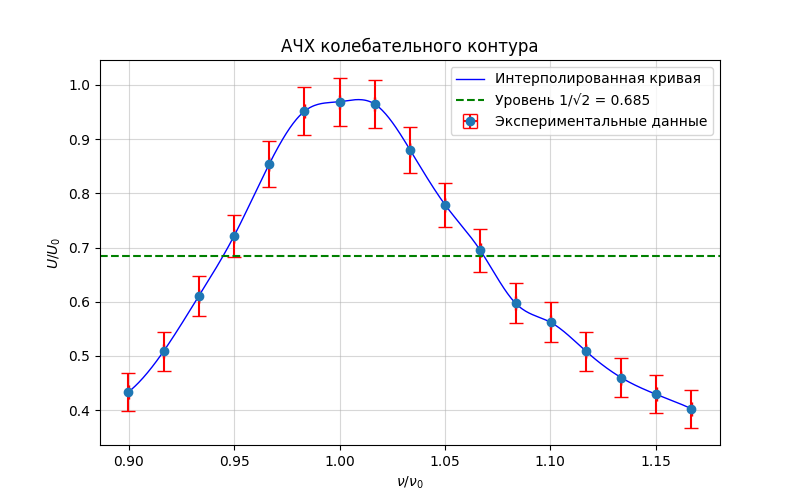
\includegraphics[width=0.81\textwidth]{Graphics/ACH_plot_final_corrected.png}}
        \caption{График 3. Амплитудно-частотная характеристика контура при $R = 382$ Ом.}
\end{figure}

\begin{figure}[h]
        \center{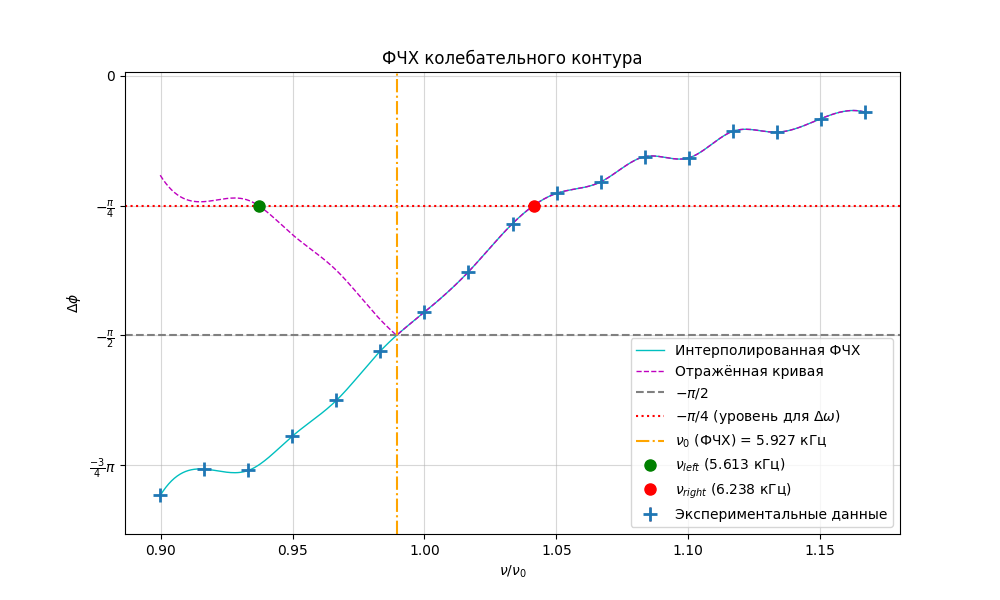
\includegraphics[width=0.81\textwidth]{Graphics/FCH_plot_detailed_method9.png}}
        \caption{График 4. Фазочастотная характеристика контура при $R = 382$ Ом.}
\end{figure}
\clearpage
\item Из АЧХ мы получили, что амплитуде $ \frac{1}{\sqrt{}2}U_0$ ($U_0 = U_{C, \text{рез}}$) соответствуют частоты $\nu_{left} \approx 5690$ Гц, $\nu_{right} \approx 6390$ Гц ($\Delta \nu \approx 700$ Гц).  $Q = \frac{\nu_0}{2 \Delta \nu} \approx 8,56$.

\item На ФЧХ мы отразили график от прямой $\Delta \varphi = -\frac{\pi}{2}$ и нашли пересечения нашей и отраженной зависимости с прямой $\Delta \varphi = -\frac{\pi}{4}$. Получили $\nu_{left} \approx 5613$ Гц, $\nu_{right} \approx 6238$ Гц ($\Delta \nu \approx 785$ Гц).  $Q = \frac{\nu_0}{\Delta \nu} \approx 9,49$.

\end{enumerate}


\section{Результаты и обсуждения}

В данной работе были проведены следующие наблюдения и измерения:
\begin{enumerate}
\item Меняя ёмкость конденсатора, замерили периоды колебаний контура. По этим данным построили зависимость $T_{\text{эксп}} = k  \cdot T_{\text{эксп}}$, получили $k = 1.006 \pm 0.006$ ($\varepsilon_k = 0,57 \%$), что подтверждает формулу Томсона $T = 2\pi \sqrt{LC}$.
\item Оценили экспериментально критическое сопротивление контура, когда система переходит в апериодический режим. $R_{\text{cr}} \approx 7 $ ÷ $ 8$ кОм.
\item Меняя сопротивление контура, измерили амплитуды колебаний.  С помощью этих данных вычислили декремент затухания и добротность (см. таблицу 2). С помощью графика $\frac{1}{\Theta^2}(\frac{1}{R_\Sigma^2})$ вычислили критическое сопротивление $R_\text{кр} = 7450 \pm 219$ Ом ($\varepsilon_{R_\text{кр}} = 2,94 \%$, теоретическое значение $R_{\text{cr}} = 2\sqrt{\frac{L}{C^*}} = 8168 \text{ Ом}$).
\item Получили спираль на фазовой плоскости на осциллографе. По ней для нашего диапазона сопротивлений получили декременты и добротность (см. таблицу 3).
\item Получили АЧХ и ФЧХ колебательного контура для $R = 382$ Ом. Добротность вычисленная по АЧХ: $Q \approx 8,56$, по ФЧХ: $Q \approx 9,49$.

\begin{table}[h!]
    \centering
    \begin{tabular}{|c|c|c|c|c|c|c|}
        \hline
        $R_\Sigma,\ \Omega$ &
        $f(L, C, R)$ &
        $f(\Theta)$ &
        $f(\Theta)$, фаз. пл-ть &
        АЧХ &
        ФЧХ \\ \hline
        382 &
        $10{,}691 \pm 0{,}012$ &
        $9{,}56 \pm 0{,}94$ &
        $8{,}91 \pm 0{,}85$ &
        8{,}56 &
        9{,}49 \\ \cline{1-4}
        592 &
        $6{,}899 \pm 0{,}008$ &
        $6{,}46 \pm 0{,}88$ &
        $5{,}96 \pm 0{,}55$ &
        & \\ \cline{1-4}
        872 &
        $4{,}684 \pm 0{,}005$ &
        $5{,}39 \pm 1{,}06$ &
        $4{,}13 \pm 0{,}40$ &
        & \\ \cline{1-4}
        1232 &
        $3{,}315 \pm 0{,}004$ &
        $3{,}86 \pm 0{,}99$ &
        $2{,}80 \pm 0{,}20$ &
        & \\ \cline{1-4}
        1632 &
        $2{,}502 \pm 0{,}003$ &
        $3{,}14 \pm 0{,}79$ &
        $2{,}27 \pm 0{,}24$ &
        & \\ \cline{1-4}
        1782 &
        $2{,}292 \pm 0{,}003$ &
        $2{,}17 \pm 0{,}48$ &
        $2{,}07 \pm 0{,}13$ &
        & \\ \hline
    \end{tabular}
    \caption{Таблица 5. Сравнение добротности контура, определённой различными методами.}
    \label{tab:q_comparison_final}
\end{table}

\end{enumerate}

\section{Выводы}

В ходе работы были исследованы свободные и вынужденные колебания в RLC-контуре. Подтверждена зависимость периода колебаний от ёмкости, определены логарифмический декремент затухания, критическое сопротивление и добротность контура различными методами. Экспериментальные данные согласуются с теоретическими предсказаниями в пределах погрешностей измерений.

\end{document}